\documentclass{standalone}
\usepackage{tikz}
\begin{document}
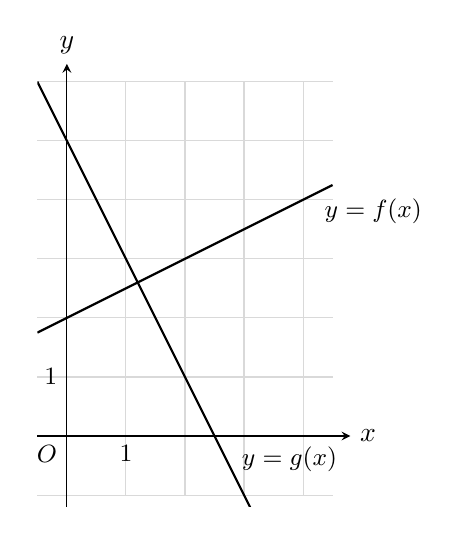
\begin{tikzpicture}[>=stealth, scale=0.75]
  % Light grid
  \draw[gray!30] (-0.5,-1) grid[step=1] (4.5,6);

  % Axes
  \draw[->] (-0.5,0) -- (4.8,0) node[right] {$x$};
  \draw[->] (0,-1.2) -- (0,6.3) node[above] {$y$};

  \begin{scope}
    \clip (-0.5,-1.2) rectangle (4.8,6.2);
    % f(x) = x/2 + 2  (slope 1/2, through (2,3))
    \draw[thick] (-0.5,1.75) -- (4.5,4.25);
    % g(x) = -2x + 5  (slope -2, through (2,1))
    \draw[thick] (-0.5,6) -- (3.5,-2);
  \end{scope}

  % Function labels
  \node[right,font=\small] at (4.2,3.8) {$y = f(x)$};
  \node[right,font=\small] at (2.8,-0.4) {$y = g(x)$};

  % Axis labels
  \node[below left,font=\small] at (0,0) {$O$};
  \node[below,font=\small] at (1,0) {$1$};
  \node[left,font=\small]  at (0,1) {$1$};
\end{tikzpicture}
\end{document}
